\documentclass[border=5pt]{standalone}
\usepackage{tikz}
\usepackage{xcolor}

\definecolor{danger}{RGB}{220,53,69}
\definecolor{warning}{RGB}{255,193,7}
\definecolor{secondary}{RGB}{108,117,125}
\definecolor{success}{RGB}{40,167,69}
\definecolor{primary}{RGB}{0,123,255}

\begin{document}
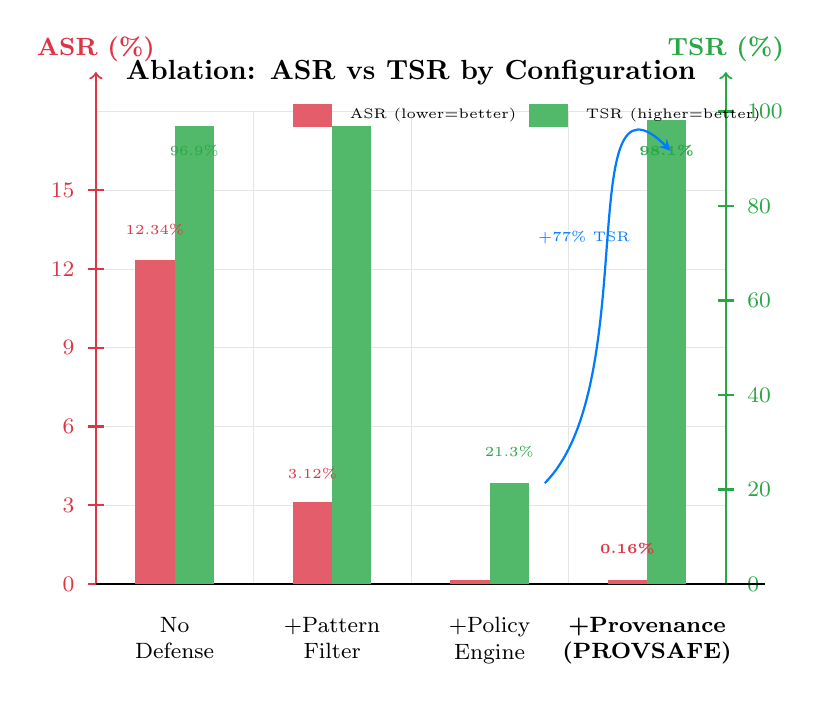
\begin{tikzpicture}[scale=1]
  % Title
  \node[font=\bfseries] at (4, 6.5) {Ablation: ASR vs TSR by Configuration};
  
  % Background grid
  \draw[gray!20, very thin] (0,0) grid[xstep=2, ystep=1] (8,6);
  
  % Y-axes
  % Left Y-axis (ASR %)
  \draw[thick, ->, danger] (0,0) -- (0,6.5) node[above, font=\small\bfseries, danger] {ASR (\%)};
  \foreach \y/\label in {0/0, 1/3, 2/6, 3/9, 4/12, 5/15} {
    \draw[thick, danger] (-0.1,\y) -- (0.1,\y);
    \node[left, font=\footnotesize, danger] at (-0.15,\y) {\label};
  }
  
  % Right Y-axis (TSR %)
  \draw[thick, ->, success] (8,0) -- (8,6.5) node[above, font=\small\bfseries, success] {TSR (\%)};
  \foreach \y/\label in {0/0, 1.2/20, 2.4/40, 3.6/60, 4.8/80, 6/100} {
    \draw[thick, success] (7.9,\y) -- (8.1,\y);
    \node[right, font=\footnotesize, success] at (8.15,\y) {\label};
  }
  
  % X-axis
  \draw[thick] (0,0) -- (8.5,0);
  
  % Bar positions
  \def\barwidth{0.5}
  
  % No Defense: ASR=12.34%, TSR=96.88%
  % ASR: 12.34/3 = 4.11; TSR: 96.88/100*6 = 5.81
  \fill[danger!80] (1-\barwidth, 0) rectangle (1, 4.11);
  \fill[success!80] (1, 0) rectangle (1+\barwidth, 5.81);
  \node[below, font=\footnotesize, align=center] at (1, -0.3) {No\\Defense};
  
  % Pattern Filter: ASR=3.12%, TSR=96.88%
  % ASR: 3.12/3 = 1.04; TSR: 5.81
  \fill[danger!80] (3-\barwidth, 0) rectangle (3, 1.04);
  \fill[success!80] (3, 0) rectangle (3+\barwidth, 5.81);
  \node[below, font=\footnotesize, align=center] at (3, -0.3) {+Pattern\\Filter};
  
  % Policy-Only: ASR=0%, TSR=21.25%
  % ASR: 0; TSR: 21.25/100*6 = 1.28
  \fill[danger!80] (5-\barwidth, 0) rectangle (5, 0.05);
  \fill[success!80] (5, 0) rectangle (5+\barwidth, 1.28);
  \node[below, font=\footnotesize, align=center] at (5, -0.3) {+Policy\\Engine};
  
  % PROVSAFE: ASR=0.16%, TSR=98.12%
  % ASR: 0.16/3 = 0.05; TSR: 98.12/100*6 = 5.89
  \fill[danger!80] (7-\barwidth, 0) rectangle (7, 0.05);
  \fill[success!80] (7, 0) rectangle (7+\barwidth, 5.89);
  \node[below, font=\footnotesize\bfseries, align=center] at (7, -0.3) {+Provenance\\(PROVSAFE)};
  
  % Annotations
  \node[font=\tiny, danger] at (1-\barwidth/2, 4.5) {12.34\%};
  \node[font=\tiny, success] at (1+\barwidth/2, 5.5) {96.9\%};
  
  \node[font=\tiny, danger] at (3-\barwidth/2, 1.4) {3.12\%};
  
  \node[font=\tiny, success] at (5+\barwidth/2, 1.68) {21.3\%};
  
  \node[font=\tiny\bfseries, success] at (7+\barwidth/2, 5.5) {98.1\%};
  \node[font=\tiny\bfseries, danger] at (7-\barwidth/2, 0.45) {0.16\%};
  
  % Arrow showing usability recovery
  \draw[thick, ->, >=stealth, primary] (5+\barwidth+0.2, 1.28) to[out=45, in=135] (7+\barwidth-0.2, 5.5);
  \node[font=\tiny, primary, above] at (6.2, 4.2) {+77\% TSR};
  
  % Legend
  \fill[danger!80] (2.5, 5.8) rectangle (3, 6.1);
  \node[right, font=\tiny] at (3.1, 5.95) {ASR (lower=better)};
  \fill[success!80] (5.5, 5.8) rectangle (6, 6.1);
  \node[right, font=\tiny] at (6.1, 5.95) {TSR (higher=better)};
  
\end{tikzpicture}
\end{document}
